\RequirePackage[l2tabu,orthodox]{nag}

% TODO: decide if one-sided/two-sided
%\documentclass[headsepline,footsepline,footinclude=false,fontsize=11pt,paper=a4,listof=totoc,bibliography=totoc,BCOR=12mm,DIV=12]{scrbook} % two-sided
\documentclass[headsepline,footsepline,footinclude=false,oneside,fontsize=11pt,paper=a4,listof=totoc,bibliography=totoc]{scrbook} % one-sided

% TODO: change citation style in settings
\PassOptionsToPackage{table,svgnames,dvipsnames}{xcolor}

\usepackage[utf8]{inputenc}
\usepackage[T1]{fontenc}
\usepackage[normalem]{ulem}
\usepackage[sc]{mathpazo}
\usepackage[ngerman,american]{babel}
\usepackage[autostyle]{csquotes}
\usepackage[%
  backend=biber,
  url=false,
  style=numeric,
  maxnames=4,
  minnames=3,
  maxbibnames=99,
  giveninits,
  uniquename=init]{biblatex} % TODO: adapt citation style
\usepackage{graphicx}
\usepackage{scrhack} % necessary for listings package
\usepackage{listings}
\usepackage{lstautogobble}
\usepackage{tikz}
\usepackage{pgfplots}
\usepackage{pgfplotstable}
\usepackage{booktabs}
\usepackage[final]{microtype}
\usepackage{caption}
\usepackage[hidelinks]{hyperref} % hidelinks removes colored boxes around references and links
\usepackage{verbatim}

\bibliography{libraries/bibliography,libraries/p2p,libraries/decentral-analyzis,libraries/other, libraries/wifi-and-cell-tower, libraries/websites}

\setkomafont{disposition}{\normalfont\bfseries} % use serif font for headings
\linespread{1.05} % adjust line spread for mathpazo font

% Add table of contents to PDF bookmarks
\BeforeTOCHead[toc]{{\cleardoublepage\pdfbookmark[0]{\contentsname}{toc}}}

% Define TUM corporate design colors
% Taken from http://portal.mytum.de/corporatedesign/index_print/vorlagen/index_farben
\definecolor{TUMBlue}{HTML}{0065BD}
\definecolor{TUMSecondaryBlue}{HTML}{005293}
\definecolor{TUMSecondaryBlue2}{HTML}{003359}
\definecolor{TUMBlack}{HTML}{000000}
\definecolor{TUMWhite}{HTML}{FFFFFF}
\definecolor{TUMDarkGray}{HTML}{333333}
\definecolor{TUMGray}{HTML}{808080}
\definecolor{TUMLightGray}{HTML}{CCCCC6}
\definecolor{TUMAccentGray}{HTML}{DAD7CB}
\definecolor{TUMAccentOrange}{HTML}{E37222}
\definecolor{TUMAccentGreen}{HTML}{A2AD00}
\definecolor{TUMAccentLightBlue}{HTML}{98C6EA}
\definecolor{TUMAccentBlue}{HTML}{64A0C8}

% Settings for pgfplots
\pgfplotsset{compat=newest}
\pgfplotsset{
  % For available color names, see http://www.latextemplates.com/svgnames-colors
  cycle list={TUMBlue\\TUMAccentOrange\\TUMAccentGreen\\TUMSecondaryBlue2\\TUMDarkGray\\},
}

% Settings for lstlistings
\lstset{%
  basicstyle=\ttfamily,
  columns=fullflexible,
  autogobble,
  keywordstyle=\bfseries\color{TUMBlue},
  stringstyle=\color{TUMAccentGreen}
}


% TODO: change thesis information
\newcommand*{\getUniversity}{Technische Universität München}
\newcommand*{\getFaculty}{Department of Informatics}
\newcommand*{\getTitle}{Crowdsourcing mobility data with privacy preservation through decentralized collection and aggregation}
\newcommand*{\getTitleGer}{Crowdsourcing von Mobilitätsdaten ohne Einschränkung der Privatsphäre durch dezentrales Sammeln und Aggregieren}
\newcommand*{\getAuthor}{Simon van Endern}
\newcommand*{\getDoctype}{Bachelor's Thesis in Informatics}
\newcommand*{\getSupervisor}{Prof. Dr.-Ing. Jörg Ott}
\newcommand*{\getAdvisor}{Trinh Viet Doan}
\newcommand*{\getSubmissionDate}{30.06.2019}
\newcommand*{\getSubmissionLocation}{Munich}

\colorlet{punct}{red!60!black}
\definecolor{background}{HTML}{EEEEEE}
\definecolor{delim}{RGB}{20,105,176}
\colorlet{numb}{magenta!60!black}

\lstdefinelanguage{json}{
    basicstyle=\normalfont\ttfamily,
    numbers=left,
    numberstyle=\scriptsize,
    stepnumber=1,
    numbersep=8pt,
    showstringspaces=false,
    breaklines=true,
    frame=lines,
    backgroundcolor=\color{background},
    literate=
     *{0}{{{\color{numb}0}}}{1}
      {1}{{{\color{numb}1}}}{1}
      {2}{{{\color{numb}2}}}{1}
      {3}{{{\color{numb}3}}}{1}
      {4}{{{\color{numb}4}}}{1}
      {5}{{{\color{numb}5}}}{1}
      {6}{{{\color{numb}6}}}{1}
      {7}{{{\color{numb}7}}}{1}
      {8}{{{\color{numb}8}}}{1}
      {9}{{{\color{numb}9}}}{1}
      {:}{{{\color{punct}{:}}}}{1}
      {,}{{{\color{punct}{,}}}}{1}
      {\{}{{{\color{delim}{\{}}}}{1}
      {\}}{{{\color{delim}{\}}}}}{1}
      {[}{{{\color{delim}{[}}}}{1}
      {]}{{{\color{delim}{]}}}}{1},
}

\begin{document}

% Set page numbering to avoid "destination with the same identifier has been already used" warning for cover page.
% (see https://en.wikibooks.org/wiki/LaTeX/Hyperlinks#Problems_with_Links_and_Pages).
\pagenumbering{alph}
\input{pages/cover}

\frontmatter{}

\input{pages/title}
\input{pages/disclaimer}
\addcontentsline{toc}{chapter}{Acknowledgments}
\thispagestyle{empty}

\vspace*{20mm}

\begin{center}
{\usekomafont{section} Acknowledgments}
\end{center}

\vspace{10mm}

I would like to thank my supervisor Prof. Dr.-Ing. Jörg Ott for allowing me to write this thesis at his chair. Furthermore, I am grateful to my advisor Trinh Viet Doan, for motivating me and for lending me their expertise and knowledge.

\vspace{10mm}

\cleardoublepage{}
\chapter{\abstractname}

We propose a method to publish location ata without raising privacy concerns.
%TODO: Abstract



\microtypesetup{protrusion=false}
\tableofcontents{}
\microtypesetup{protrusion=true}

\mainmatter{}

% !TeX root = ../main.tex
% Add the above to each chapter to make compiling the PDF easier in some editors.

\chapter{Introduction}\label{chapter:introduction}
\section{Why we need an open-source location data approach}\label{chapter:introduction:section:motivation}

%\subsection{General motivation: We want to open-source data} \label{general-motivation}
“Data is the new oil” is a quote many people agree with. It means that more and more businesses are
based not on specific production capacities but on data, the ability to process it and the exclusive owenership over it. The success and monopoly of
companies like Google, Facebook and Amazon can be attributed to this exclusive ownership to a significant extend.

While patents that used to power companies' success provide a balance through granting exclusive rights while having to make the knowledge public, many companies e.g. Coca cola have decided successfully not to go for a patent and thus not reveal their knowledge. If that approach is not compromised, it guarantees both - non-disclosure and also exclusive rights. Similarly, the non-disclosure of huge data sets collected by Facebook, Google and Amazon circumvent the balance intended by patents. The unavailability of huge amounts of data to the public is an impediment of innovation and increased growth. For example, cities would benefit from aggregated location data in order to optimize traffic scheduling as also highlighted by \parencite{hoh2005protecting}.
Nevertheless, the publication of raw data sets is impossible because it severly intrudes the privacy of the owners of the data.\\

%\subsection{Main problem: Conflict between privacy and publishing user data}
So, even if companies would agree on a publication, a problem arises.
There is a conflict between preserving user privacy and publishing user data.\\

%\subsection{Existing privacy problem: The availability of central data sets}
Nevertheless, user privacy is already compromised even without publication of user data.
Already the mere existence of central data sets pose a privacy risk to users, because security issues might allow for theft and unwanted publication of these data.
An example is the theft of 14 million user data from facebook \parencite{facebook}.\\

%\subsection{Relaxed privacy problems: The limited but not eliminated risk through a modified central data set}
Some governments and other institutions already publish some of their data sets after anonymizing them e.g. through cloaking of data so that it achieves k-anonymity and there are crowdsourcing and open source approaches to make data available to everybody. 
Nevertheless, the applied anonymization is often not sufficient or at least critical if the resulting data set should still be useful. Research shows that inferences can be drawn from the published data sets that violate the respecitve users' privacy. So, in addition to the main risk of a central data set, publishing anonymized data poses another risk to users privacy.\\

%\subsection{New problem in case of modified central data set: Trust to the server is needed}
Furthermore, besides the remaining risk of inference attacks in published anonymized data sets, the anonymization through those algorithms always depend on a trusted server to collect the data from all users and then publish the results of any analysis applying privacy-preserving algorithms beforehand. So even if the data is only stored anonymized on the server, besides the remaining risk of inference attacks, this still imposes a high privacy risk to every user, as trust can be misued by the trusted server itself.\\

\section{Research Question: No central raw data set but only aggregated data}
RQ 1: What features does such a system require?
RQ2: ...
Nach dem Stil.


Clearly, in order to overcome the conflicit between privacy intrusion and (public) data availability, a solution is needed that gets along without storing raw data in a central data set.
This solution should 1. eliminate the risk of leaking raw user data through theft from a centralized database and 2. eliminate the remaining risk of inference attacks on published believed-to anonymized raw data. So far, we have not seen an approach to fully solve this problem.\\

\section{Contributions}
For our solution, we will focus on the sub-area of location data and location privacy.
We investigate the possibility of storing raw location data only decentralized on the collecting devices. On a central server available to the public, only aggregated data is stored, thus the main problem of privacy risk by a central database containing the overall raw data set is solved. Furthermore, the issue of trust is removed, as the aggregation process happens decentrally, thus the central server will never hold any other data than aggregated data. It will never know about the individual raw data.

In summary, our approach takes the opposite direction as todays standard. We do not first collect the whole data set and then reduce it to a data set meeting privacy-constraints but we start from the bottom up - first by performing analysis in a decentralized manner so that there never is an overal data set imposing a security risk on all the entries' users, and second by proposing a framework that only releases aggregated data where no interference of any user information is possible. This data will then be available to the public. This gives us maximum possible feedback on eventual privacy problems, creates trust through transparency and fosters innovation through availability of data to everyone.

%and supports the process of not randomly collecting data and afterwards researching on metrics that are actually needed but first on evaluating which metrices are needed and then retrieving them if possible without raising privacy concerns.

\section{Outline}
The structure of our research is organized as follows: First we re-
view related work in the areas of location privacy and anonymisation techniques. In
section \ref{chapter:solution} we describe our approach of decentralized data analysis to get along without a central database.
Section XXX describes the setup in detail. Section XXX analysis the result from field-testing our application.
Section XXX incorporates the results into our proposal of a possibility to achieve 100\% privacy through all applications.
Section XXX summarizes our work and points out further research possibilities.

%The rest of this research is organized as f

%But also privacy concerns of users have increased due to leakages where their data was not well protected at e.g. facebook and stolen and published.



%So, we identify two related issues compromising data privacy. 
%\begin{enumerate}
%  \item The availability of huge data sets at central servers imposes a risk stemming from the computer science area of security. (main risk)
%  \item Publication of entire data sets can even after applying anonymization techniques not guarantee privacy preservation. (reduced risk)
%\end{enumerate}

%\subsection{Examples of direct and indirect privacy breaches}


%An example for the second issue is that the location data of Twitter tweets was published without asking the user for permission. Furthermore this data is only available through the API, so that the user is not aware of this infringement. Using this data, ~\parencite{twitter} has shown that this data can be used to infer a users home address and often also the work address, even if the user itself is privacy-aware, thus does not publish his / her name, etc.



%\begin{itemize}
%  \item Collect less data \parencite{privacy-home-work-pairs}
%  \item Mixing approach \parencite{location-privacy}
%  \item Anonymize data to meet the kriteria of k-anonymity \parencite{k-anonymity} and \parencite{cellphone}
%  \item spatial cloaking \parencite{krumm}
%  \item Remove not only identifiers from the data set but also apply algorithms, that remove samples, that can be (due to few samples in this area) identified \parencite{time-to-confusion}
%\end{itemize}

%\subsection{Problems that still arise}

%Still this privacy is only limited if only this one data set is taken into account. If e.g. multiple of those data sets from different data collectors are combined, or information about an individual like home and work adress is provided, privacy breaches are still highly likely.




% !TeX root = ../main.tex
% Add the above to each chapter to make compiling the PDF easier in some editors.
\chapter{Related Work}\label{chapter:related-work}

\section{Classification of location data usage according to acceptable delay}
In order to review existing approaches and research, we classify location aware services by the acceptable delay of the location information being available. Similar to the classification implied by Hoh et al. \parencite{hoh2005protecting} and Gruteser et al. \parencite{gruteser2003anonymous}, we define three categories:
\begin{enumerate}
  \item \textbf{Almost no delay tolerance:} e.g. an application showing a pop-up about a nearby venue e.g. a coffe shop when a pedestrian passes by.
  \item \textbf{Some delay tolerance e.g. one minute:} An application e.g. google maps derives the information of congested traffic from devices reporting their GPS data which show lower than usual speed on the respective road. As congestions worth reporting last longer than one minute, some delay in the device's information reaching the server is acceptable.
  \item \textbf{Significant delay tolerance of hours, days or even weeks:} For historical and statistical use of location data e.g. to find out about popular visiting times of a venue, almost any delay is acceptable.
\end{enumerate}
Some research deals with category one where almost no delay tolerance is acceptable \parencite{location-privacy, mix-zones, tang2006putting}. For example, Tang et al. \parencite{tang2006putting} propose a possibility to collect data about the number of people currently at a venue through the number of devices registered in the respective WIFI. This data is collected by a client application and anonymously send to a central server. Mokbel et al. \parencite{casper} and Tang et al. \parencite{tang2006putting} propose a solution where not the exact location is send to a server but the rough region of the user. The server then sends a list of all possible matches e.g. petrol stations in this area to the client. Locally, this list is then matched with the exact location in order to fulfill the aim of the respective application.
Most research though investigates users' privacy for category 3 where the delay of the data being available for processing is not an issue \parencite{krumm, cellphone, privacy-home-work-pairs, twitter}. In the following, we will concentrate on this case as well.
%review research tackling location privacy in case 3 and 2 and then briefly point out the findings for case 1.

\section{Privacy problems arising from location data}
\subsection{Risk of privacy intrusion through theft of central databases}
Centralized databases containing raw location data expose users to a privacy risk (through theft) \parencite{iot, hoh2006enhancing}. Jabbar et al. \parencite{p2p-android} proposes the use of P2P over WIFI and Bluetooth to decrease the need of central instances. Nurminen et al. \parencite{nurminen2006p2p} uses SMS and highlights possibilities to switch to IP once a connection is build up. A decentralized analysis approach and it's implications for data privacy is also investigated by Stolpe \parencite{iot} as an alternative to cloud-based IoT.
Kajino et al. \parencite{crowdsourcing} proposes an approach for crowdsourcing in which raw data is hidden from the central instance but still aggregated data can be obtained by using encryption methods. Raw data is encrypted using a modified approach of public-private key-pair cryptography in which the sum of two encrypted messages can be decrypted to the sum of the encrypted messages. Furthermore, only a number of messages above a certain threshold can be encrypted this way using the different encryption shares.
%While this approach is close to our work in general, we propose a more general and flexible setup.
Another approach by Hoh et al. \parencite{hoh2006enhancing} also uses encryption in combination with a middleware. The server storing the data and the participant (e.g. a vehicle) share a symmetric key which is stored securely in the vehicle. The middleware ensures authentication of the participant, and forwards the location to the central server without giving away the vehicle's identity. Nevertheless, several research as e.g. \parencite{krumm, twitter, cellphone} have shown that it is easy to infer identity from such data sets and thereby de-anonymize them. 
%Even though they solve the problem of user authentication, it seems hardly feasable as the symmetric key has to be pre-installed on every participating device.

\subsection{Inference attacks on published anonymized data}
Research has shown, that from a location data set that is pseudonymous, i.e. the identifiers have been stripped off or the data set has been anonymized in another way, it is possible to infer the home location of single users through so-called inference attacks \parencite{krumm, cellphone, privacy-home-work-pairs, hoh2006enhancing, twitter} and also the work location with a slightly lower probability \parencite{cellphone, privacy-home-work-pairs}. The same problem has been identified by Kajino et al. \parencite{crowdsourcing} when using data collected through crowdsourcing.
These home locations or home-work location pairs can then be used to look up the corresponding user's identity e.g. by combining it with publicly available information. One possibility is to reverse code GPS coordinates to addresses and then e.g. search for entries in telephone books to infer the user's identity from it's home location \parencite{krumm, privacy-home-work-pairs, hoh2006enhancing}. Especially in suburban areas this is quite successful as usually one house can be mapped to only one person or family. This identity can then be linked to other sensitive data, e.g. locations visited by the identified user. The same problem also arises in the area of IoT \parencite{iot, hoh2006enhancing}.

\section{Countermeasures to prevent inference attacks}
In general, it has been found by Sweeney et al. \parencite{k-anonymity} that the problem can be solved by providing k-anonymity for the data set. A data set is k-anonymous, if querying for an identifier in this data set always returns a result set of at least k entries.
In order to achieve this, several approaches have been investigated. Krumm \parencite{krumm} and Xu et al. \parencite{xu2018location} and Gruteser et al. \parencite{gruteser2003anonymous} propose spatial cloaking. K-anonymity is achieved by dropping data points or perturbing them or dropping all data points around a random point around the home location. Also obfuscating locational data (close to a home location) and mapping GPS points to the next street crossing or only sending e.g. the city or department instead of the exact location is possible to increase anonymity.
More sophisticated approaches as e.g. by Hoh et al. \parencite{time-to-confusion} focus on making it less likely to identify GPS points of one trajectory being subsequent and belonging to the same user.

\section{Limitations of countermeasures}
Usually there is a trade-off between the level of anonymity and the usefullness of the data. When k-anonymity is guaranteed, often the resulting data set becomes useless because the data quality is not sufficient anymore \parencite{krumm, cellphone, k-anonymity-old, k-anonymity, k-anonymity-achieving}.
On the one hand, when the data set is tried to be kept usefull, data suppression algorithms have only limited success and can only reduce, but not eliminate the risk as shown by Hoh et al. \parencite{hoh2006enhancing}. Several research \parencite{time-to-confusion, location-privacy, hoh2006enhancing} finds that anonymization techniques might score well in densly populated areas or areas with high traffic but poorly in sparsely populated areas especially where a single address can be mapped to a single person or family. Also Golle et al. \parencite{privacy-home-work-pairs} find that the applied techniques might not achieve the expected results for individuals who's work and home location are a lot further away than average.
Furthermore, Sweeney \parencite{k-anonymity-achieving} finds that taking other sources and databases into account, k-anonymity might be compromised due to quasi-identifiers e.g. a combination of attributes that do not identify an individual but allow linking two different data sets and by that creating new identifiers. Also, Xu et al. \parencite{xu2018location} find that privacy is lower, if road semantics i.e. which types of buildings e.g. hospital, supermarket, are taken into account.
Apparently, the key to a higher degree of privacy also highlighted by Chatzimilioudis et al. \parencite{chatzimilioudis2012crowdsourcing} is to strictly not publish any trajectory.

%\parencite{location-privacy, mix-zones} introduces mix-nodes, that can nevertheless not guarantee privacy and also depnds on a trusted third party.
		%Also \parencite{casper} proposes a solution (close to our summary) how to enable privacy for instant use of location data.

%Decentralized methods for data analysis are also motivated from the area of IoT \parencite{iot}.
% !TeX root = ../main.tex
% Add the above to each chapter to make compiling the PDF easier in some editors.
\chapter{Methodology}\label{chapter:method}
In order to avoid having a central raw dataset and to eliminate the risk of inference attacks on anonymized data, we propose a framework which collects and locally aggregates location data on end user devices (smartphones) through an application designed for this purpose. The raw data will stay on each device and will only be used to serve aggregation requests send from the central server. The aggregation requests have to be defined upfront. An example is the determination of the average number steps per day accross all users participating in the respective aggregation. An examplary incoming aggregation request is depicted in figure \ref{incoming-aggregation-request}. It specifies the timespan which should be covered by the aggregation and the type of aggregation.

\begin{figure}[h!]
	\begin{lstlisting}[language=json,firstnumber=1]
	{
		"start": "2019-05-30",
		"end": "2019-06-02",
		"type": "steps",
		"n" : 3,
		"value": 2000
	}
	\end{lstlisting}
	\caption{Incoming aggregation request}
	\label{incoming-aggregation-request}
\end{figure}

The response send back to the server after processing the request only needs to contain the data itself, as the type and timespan can be inferred by the server from the request identifier. Figure \ref{outgoing-aggregation-response} shows an examplary response to the server that matches the request in figure \ref{incoming-aggregation-request}.

\begin{figure}[h!]
	\begin{lstlisting}[language=json,firstnumber=1]
	{
		"n" : 4,
		"value": 2500
	}
	\end{lstlisting}
	\caption{Outgoing aggregation response}
	\label{outgoing-aggregation-response}
\end{figure}

\begin{figure}[h!]
	\caption{Decentral unencrypted aggregation process via P2P}
	\label{decentral-aggregation-unencrypted}
	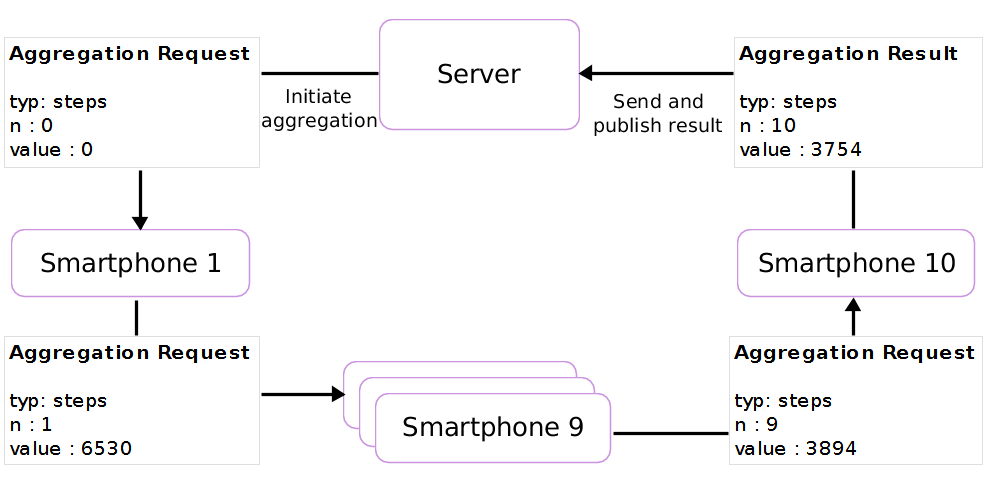
\includegraphics[width=\textwidth]{data/diagrams/decentral-aggregation-6.png}
\end{figure}

Figure \ref{decentral-aggregation-unencrypted} depicts the overal process of such a decentral aggregation request using an example of 10 participating devices.
In order to protect the user's privacy and completely shield the raw data from the server, it would be necessary to pass the request via P2P from one device to another until the last device finally sends the results to the server. P2P on mobile phones though is hardly possible, if the devices are not locally close to each other \parencite{p2p-android}. On the other hand, if the server is used to pass an aggreation request from one device to another, it could read the data and compute the respective user's input from the difference. We propose to use encryption in order to hinder the server from reading the data and assume the server to be trusted in the first place. Chapter \ref{chapter:conclusion} discusses this limitation. The modified aggregation process is depicted in figure \ref{decentral-aggregation-encrypted}. On installation of the application on a smartphone, a public-private key-pair is generated and every installed application registers at the server with this public key. The corresponding private key is stored locally. On start of an aggregation request, not only the first user but also the following user who should deal with the aggregation request is determined and the public key of the next user is passed along with the aggregation request. When one end user device needs to send the processed aggregation request to the next phone, it encrypts the data using the provided public key of the next user in the standard hybrid encryption\footnote{In hybrid encryption as used in SSL, the message itself is encrypted with a synchronous key while this key itself is encrypted using the public key} approach leveraging the benefits of synchronous keys. This way the next phone in the aggregation chain will be able to decrypt the request and process the data while the server is unable to read the data until the aggregation request is finally send in plain text for publishing to the server. This process currently assumes a trusted server and trusted devices. Chapter \ref{chapter:conclusion} discusses these limitations.

 \begin{figure}[h!]
	\caption{Decentral encrypted aggregation process}
	\label{decentral-aggregation-encrypted}
	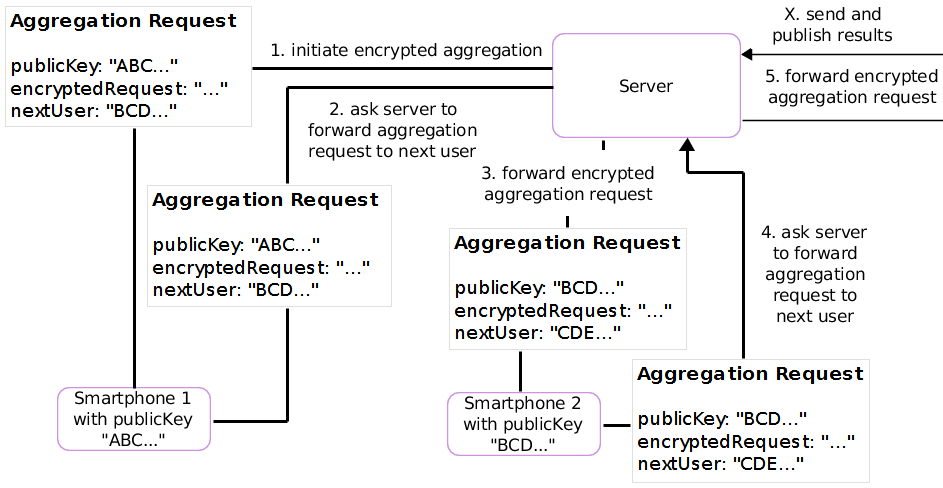
\includegraphics[width=\textwidth]{data/diagrams/decentral-encrypted-aggregation.png}
\end{figure}

 The aggregated results are planned to be available through a public route on the server. Nevertheless, we restricted access in out test run to our research team in order to protect the research participants' privacy in case there is a privacy risk we have not thought of. The aggregation requests themselves are initiated by our research team but can be initiated automatically on a regular basis in the future.

 \section{Aggregation schemes}\label{aggregation-schemes}
 Two types of aggregation requests are of special interest for our research. First, the aggregation of mean values and second, the aggregation of more advanced statistical values such as median or distribution. The latter includes the possibility to calculate the former and requires the simultaneous availability of each single user's response. %Nevertheless, we want to test all research questions independently.
 The following list is an excerpt of aggregations in the area of location data that would be of interest:
 \begin{enumerate}
 	\item Computing the average number of steps walked across all users participating in the request. (e.g. to calculate how many people reach the 10.000 steps per day\footnote{It has to be evaluated, which percentage of steps are registered because the phone will not always be on the person}.)
	\item Computing the average time spent walking, running, in a vehicle or on a bicycle.
	\item Computing how many people respectively which share of people combine using a bicycle with using a vehicle such as public transport or a car within one trajectory.
	\item How much time do people spend at work.
	\item How long do people travel to work.
	\item Where did many participants spend a significant amount of time on a certain day? (A posteriori Event recognition)
	\item What percentage of whole travelling time do people spend on their bike, car, ...
	\item What is the average speed on roads.

	\item Collecting a list of the average number of steps walked by each participant during the timespan.
	\item Collecting a list of the duration of all registered activities.

	\item collecting a list of all trajectories registered by the users' phones.
 \end{enumerate}
 For all these and more aggregations, always both, the mean value and if possible, a complete list of single users' mean values in order to compute other statistical figures, are of interest.

 \section{Limiting the spatial area of an aggregation request}
 The aggregation requests outlined in the former subsection only provide useful data if the area of the aggregation can be limited e.g. to the scope of a city. Otherwise the resulting data would not allow for comparison and the scope of each aggregation would either be the whole user base which especially in the case of listing values would result in a huge amount of data passed around. Or, the limited number of participants in each aggregation would not be locally close which would not result in useful data and also make it impossible to do aggregations as the average speed on roads, where you need a certain number of participants providing data about this area. 
 In order to limit the area of aggregation and avoid sending the aggregation request to each user and leaving him with determining whether he is inside the area and participates in the request, the initiator of those requests has to now the location of users, respectively the location where the user is active the most.
 We do not see this as a violation of the user's privacy due to the following reasons:
 \begin{enumerate}
 	\item The exact location of the user e.g. the home or work location is not of interest at all. Rather the area for which the user can provide data is of interest. We propose to cluster location areas in a hierarchical structure similar to \parencite{casper} and determine the granularity of the location published to the server as follows:
 	\begin{enumerate}
 		\item Each user sends the most coarse locational area possible to the server - e.g. the continent.
 		\item If more than the required anonymity threshold of e.g. 10 active users are already registered with this location at the server, the server not only links this location to the user but also requests the user to send a less coarse location.
 		\item The user step by step sends a less coarse location e.g country, district, etc. until the server denies the location because not enough active users have registered with the location on this granularity level. It nevertheless increases a counter of users who requested access to this location. Once the counter exceeds a certain number, the server sends an aggregation request to participants in the more coarse area encompassing the requested less coarse area to determine the number of active users. If this number is above the required threshold, the granularity level for this location is made available and users can now register with this area and aggregation requests targeting this area can be send.
 		\item The fullfilment of the threshold has to be checked on a regular basis in order to close areas once the user base sinks below the anonymity threshold.
 	\end{enumerate}
 	In a more advanced setting, it should be possible to register with more than one area on the same level to avoid that a user e.g. living close to a city provides only data about the city or the bordering area but not both. Nevertheless, this should be limited to areas bordering each other to avoid user identification similar as in XX and it has to be investigated whether this indeed does not pose a privacy risk to the user or whether also the combination of areas needs to meet a certain anonymity threshold.
 \end{enumerate}
% !TeX root = ../main.tex
% Add the above to each chapter to make compiling the PDF easier in some editors.
\chapter{Design and Implementation}\label{chapter:design}

\section{Technology Stack}
In order to implement the architecture proposed in chapter \ref{chapter:method} we chose Android as end user device platform. Android has the highest market share \cite{android-market-share} among mobile devices and offers a healthy ecosystem of frameworks and libraries that simplify development. Furthermore we opted for an implementation in Kotlin to reduce boilerplate code and improve readability.

As server side technology we chose node.js in conjunction with a mongoDB object store database. A NoSQL database like mongoDB provides flexibility and easy adaption of data schemes without much overhead and thus perfectly fits our prototyping purpose. We chose node.js out of the same reasons. In contrast to a statically typed language, javascript provides more flexibility and ease of change. Furthermore node.js is often used in combination with mongoDB and provides seamingless integration.

The results can be made available to the public either via a dedicated route of the server or directly through granting right access to the respective collection\footnote{A collection in an object store is the equivalent to a table in a SQL database} of the database.

The following sections describe the implementation of the Android application and the server and explain design decisions. We start with an outline of the API shared by the application and the server.

\section{API}\label{api}
The API is designed as a pure REST API based on JSON.
The API consists of the following endpoints:
\begin{itemize}
	\item POST /user - for creating a new user
	\item GET /requests?pk=... - for retrieving aggregation requests for a user
	\item POST /forward - for sending a processed aggregation request back to the server
	\item GET /aggregations - for retrieving all completed aggregation results
	\item POST /admin/sampleRequest - for starting a new aggregation request.
\end{itemize}
\begin{figure}[h!]
\begin{lstlisting}[language=json,firstnumber=1]
{
  "publicKey": "-----BEGIN PUBLIC KEY-----\nMIIBIjANBgkqhkiG..."
}
\end{lstlisting}
\caption{POST /user}
\label{post-user-request}
\end{figure}

\begin{figure}[h!]
\begin{lstlisting}[language=json,firstnumber=1]
{
  "publicKey": "-----BEGIN PUBLIC KEY-----\nMIIBIjANBgkqhkiG...",
  "password": "LSFDfzduSFSozfwf"
}
\end{lstlisting}
\caption{Response to POST /user}
\label{post-user-response}
\end{figure}

\begin{figure}[h!]
\begin{lstlisting}[language=json,firstnumber=1]
[{
  "publicKey": "-----BEGIN PUBLIC KEY-----\nMIIBIjANBgkqhkiG...",
  "serverId": "5cfbd6734e733a0079ee5c0f",
  "nextuser" : "-----BEGIN PUBLIC KEY-----\nMIIBIjANBgkqhBms...",
  "encryptionKey":"HXporX7tqrgkf6Cp8OlqOcpLb...",
  "iv":"pMxQ2nHqbz1Zu24Lfi5HYQ==",
  "encryptedRequest":"xtgP2e9AeAK8hfPXQe03..."
}]
\end{lstlisting}
\caption{GET /requests}
\label{get-requests-request}
\end{figure}
POST /forward:
\begin{figure}[h!]
\begin{lstlisting}[language=json,firstnumber=1]
{
  "publicKey": "-----BEGIN PUBLIC KEY-----\nMIIBIjANBgkqhkiG...",
  "password": "LSFDfzduSFSozfwf",
  "serverId": "5cfbd6734e733a0079ee5c0f",
  "encryptionKey":"HXporX7tqrgkf6Cp8OlqOcpLb...",
  "iv":"pMxQ2nHqbz1Zu24Lfi5HYQ==",
  "encryptedRequest":"xtgP2e9AeAK8hfPXQe03..."
}
\end{lstlisting}
\caption{Response to GET /requests}
\label{get-requests-response}
\end{figure}

\begin{figure}[h!]
\begin{lstlisting}[language=json,firstnumber=1]
[{
  "timestamp": 1559216514521,
  "startedAt": 1559216514685,
  "start": "2019-05-28",
  "end": "2019-05-31",
  "type": "steps",
  "n": 6,
  "value": 4271,
  "valueList": []
},
{
  "timestamp": 1559216514521,
  "startedAt": 1559216514685,
  "start": "2019-05-28",
  "end": "2019-05-31",
  "type": "stepsListing",
  "n": 5,
  "value": 0,
  "valueList": [1661, 1246, 3195, 7714, 7842]
 }]
\end{lstlisting}
\caption{Response to GET /aggregations}
\label{get-aggregations}
\end{figure}

POST: /admin/insertSample
\begin{figure}[h!]
\begin{lstlisting}[language=json,firstnumber=1]
[{
  "password": "adminPassword",
  "start": "2019-05-31",
  "end": "2019-06-05",
  "type": "activity_2",
}]
\end{lstlisting}
\caption{POST /admin/insertDample}
\label{insert-sample}
\end{figure}

TODO: Password should go into header in the future.

The routes used for interaction with the application (see figures \ref{get-requests-request} and \ref{get-requests-response}) (except the one for creating a new user (see figures \ref{post-user-request} and \ref{post-user-response})) are secured and can only be used if the users can successfully be authenticated. The routes for starting new aggregation requests (see figure \ref{insert-sample}) and retrieving all results require administrator authentication. The route for the results (see figure \ref{get-aggregations}) is designed to be available to the public without authentication. Nevertheless we restrict access only to result types that have been examined to fully protect users' privacy. So, for example, our experimental trajectory request type is not available to the public.

The encryptedRequest as of figure \ref{get-requests-response} contains the encrypted version of the request described in the following subsection.

//TODO: Integrate this section somewhere else (in methodology)
\subsection{Data Aggregation Design}
All aggregations proposed in section \ref{aggregation-schemes} can be implemented using only 4 fields: An integer \textit{n} specifying the current number of participants, A Floating Point Number \textit{value} e.g. containing the current mean value of the aggregation, a list \textit{valueList} of Floating Point Numbers that can be reused for different purposes accross requests and a \textit{type} field that specifies the request and the scheme how the other fields are populated e.g. the encoding of the \textit{valueList}

All aggregation requests have a start day and an end day in common. Days' time is always treated as 00:00 o'clock. Thus, the timespan for an aggregation is always a multiple of 24 hours.
Due to limited scope of this thesis, only the following out of the aggregation requests defined in section \ref{aggregation-schemes} were implemented:
\begin{enumerate}
	\item Computing the average number of steps walked across all users participating in the request.
	\item Computing the average time spent walking, running, in a vehicle or on a bicycle\footnote{https://developers.google.com/android/reference/com/google/android/gms/location/DetectedActivity}.
	\item Collecting a list of the average number of steps walked by each participant during the timespan.
	\item collecting a list of all trajectories registered by the users' phones.
\end{enumerate}

Aggregation 1 and 2 are implemented in order to answer research question 1. Aggregation 3 was implemented to especially to test research question 2.
%whether this type of aggregation, which allows for more advances statistical computations as median values and distribution properties, still completely preserves privacy.
Aggregation 4 imposes a privacy risk discussed in \parencite{twitter, cellphone, krumm} on the user and was implemented in order to get an overview of the data quality of our setup and validate the feasability of the other aggregation requests proposed in section \ref{aggregation-schemes}.

\section{Android Application}
The Android application targets Android Oreo (API level 27) and requires a minimum API level of 19. Approximately 96.8\% of devices run on this or a higher version of Android \cite{android-api-level-share} which allows our application to be installed on the majority of Android devices.
Furthermore, the application leverages Goolge Play Services to obtain GPS and activity data. Without Google Play Services installed, the application will not work. In order to ease future adaptability, we chose to use the Dagger2\footnote{https://dagger.dev/} framework for dependency injection in order to decouple classes as far as possible. Further use of frameworks and libraries will be explained in the following respective sections.

Th application is aimed to collect GPS data, detect the user's current activity and count the user's steps. The data collection process happens in the background without any user interaction needed. Aggregation requests to aggregate data accross devices are also served without any user interaction needed.
The android application can be grouped into three main parts of loosely coupled modules:
\begin{itemize}
	\item A module responsible for collecting and saving raw data
	\item A module responsible for locally aggregating raw data
	\item A module responsible for communicating with the server and handling aggregation requests
\end{itemize}

\begin{figure}[h!]
  \caption{Android architecture}
  \label{android-overview}
  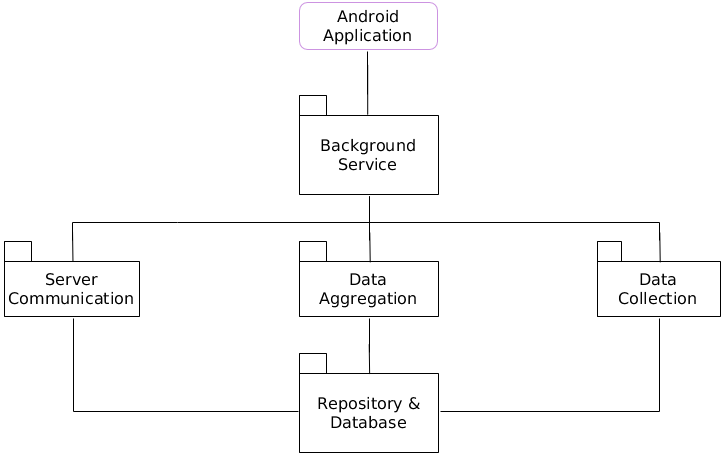
\includegraphics[width=\textwidth]{data/diagrams/android-architecture.png}
\end{figure}

The control flow as depicted in figure \ref{android-overview} is as follows: 
The application has only one Main Activity in order to ask the user to allow location access and start the background services. Apart from that the only Activity does not serve any specific purpose. 
The local aggregation as well as the polling of new requests from the server happens in the background on a 15 minute interval. The Android Workmanager controls this periodic work without any user interaction being required.

For the App in order to have maximum possibilities collecting esspecially GPS data and preventing the Android operating system from shutting down when not interacted with by the user (which is usually never the case), a non-dismissible status notification is displayed at all time. (Compare to the non-dismissible status notification displayed by Google Maps when the navigation system is active). Also the application is registered to be automatically restarted upon boot\footnote{From Android 6.0 on (API level 23), restricts apps' behaviour in order to reduce battery consumption. E.g. all apps are automatically managed by the battery manager which restricts background launches. The user has to switch this option to manual management in order to allow the app to function in the way it was designed. See https://developer.android.com/guide/background/ and also https://developer.android.com/training/monitoring-device-state/doze-standby} and also when the application is closed by the user (e.g. via the task manager) so that once installed, no further user interaction is necessary.
Furthermore, the application, respectively each module is heavily unit tested in norder to guarantee functionality and facilitate further development by other research teams. Unit and integration tests are based on AndroidJUnit4 and the expresso\footnote{https://developer.android.com/training/testing/espresso} framework.

\subsection{Separation of concerns regarding Data Collection and Aggregation}
We choose to separate the aggregation and collection of location data in order to decouple the modules and provide the possibility to extend the model of aggregated data in the future without the need to change the raw data model. Vice versa the data collection process can be modified without impacting the aggregation process.

\subsection {Data Collection}
We use the Android Room Persistence library\footnote{https://developer.android.com/topic/libraries/architecture/room} to locally store data. The library provides a layer over the standard LiteSQL database commonly used in many Android applications. We collect three types of data:
\begin{itemize}
	\item Steps: If available, the phone's internal step sensor provides updates on a regular basis. The step sensor always informs about the total number of steps since the last reboot. Upon each time we receive data from the step sensor, this data is stored directly in the \textit{step\_counter\_table}.
	\item User's activities: The Google Play Services  activity recognition API leverages different data and sensors available on the phone in order to inform about the most probable current activity of the user as one of \textit{still, walking, running, in a vehicle, on bicycle}. Whenever there is a change detected, two events are fired - one for exiting the former and one for entering the current activity. The events might not be dispatched instantly but contain the timestamp of the exact occurence. Upon each received event, this data is stored directly in the \textit{activity\_transition\_table}.
	\item GPS positions: GPS data is retrieved through the \textit{FusedLocationProviderClient} which leverages cellphone-tower and WIFI data apart from GPS to determine the position. In order to limit battery consumption, GPS data is only requested every minute if the device's detected activity is \textit{still}\footnote{Neertheless, if other applications request a GPS position, our application also receives this data, even if it occurs on a faster interval}. If the current detected activity is \textit{walking}, the interval is set to 5 seconds and in any other state, the interval is set to every second. The data is stored in the linked tables \textit{gps\_data\_table} and \textit{gps\_location\_table}. We choosse to separate the GPS point itself from the timestamp having in mind that future aggregations might need or leverage the separation of spatial data and time and more than one event might be attached to the same GPS point.
\end{itemize}

\subsection{Local Data Aggregation}\label{local-data-aggregation}
From the received values of the step counter since last reboot saved in \textit{step\_counter\_table} the daily steps are computed and stored in \textit{steps\_table}. The exit and enter events received via the activity recognition framework and stored in the \textit{activity\_transition\_table} are matched in order to compute activities with start and duration. Those activities are then saved in the \textit{activity\_table}.
GPS data is used to compute trajectories through the following algorithm:
\begin{enumerate}
	\item When there are more than 10 minutes between two subsequent GPS points in the sequence of all GPS points to be processed, the sequence is separated into two separate sequences and each is processed separately as a possible trajectory in the next step.
	\item First, we identify still moments - periods of no movement - as follows:
	\begin{enumerate}
		\item For each GPS point, we identify a subsequent GPS point that was registered at least two minutes after the first one.
		\item If the average speed between those two points was below 0.6 m/s, the pair is added to a list to be processed in the next step.
		\item The list of pairs of GPS points resulting from the last step is fused into sequences of GPS points as long as possible: Whenever two pairs overlap in their timestamp, they are fused to a new pair covering the combined timespan.
	\end{enumerate}
	\item The resultig GPS pairs of still moments are used to exclude still moments from the original sequence and divide it into subsequences marking trajectories.
\end{enumerate}
Of each trajectory, the start and end location as well as the respective timestamp are then saved in \textit{trajectory\_table}. We tested 0.5 m/s, 0.6 m/s and 0.7 m/s as threshold in step 2b) and found 0.6 m/s to be best fit the tested sample. On the one hand the threshold must be low enough to still include slow walking which might be below 1 m/s. On the other hand, the threshold should not be too low because inaccuracy in GPS data might otherwise induce trajectories where the device has actually not moved at all.

Example of algorithm (TODO):
\begin{verbatim}
{
	Original dataset:			
	Latitude Longitude Time
	44		 11		   10:11:03
	44.5	 11.1	   10:11:15
	44.4	 11.05	   10:12:12
	44.3	 11.07	   10:33:00
	44	     11.2	   10:34:00
}
\end{verbatim}

\subsection{Serving Aggregation Requests}
We use the retrofit2 framework\footnote{https://square.github.io/retrofit/} based on OKHTTP\footnote{https://square.github.io/okhttp/} to handle communication with our REST server dexribed in \ref{server}. An HTTP Interceptor is used to modify incoming and outgoing requests. The interceptor decrypts the request body of incoming messages using the private key of the installation before the body is parsed into Java Objects. On outgoing messages the inteerceptor adds authentication before sending them to the server.
The app polls for new aggregation requests every 15 minutes. New aggregation requests are first stored locally in the database. Those requests are then processed and the results are again stored locally as pending outgoing requests until they are finally send to the server. Figure XX illustrates this process. This separation of concerns is useful especially in case of an interrupted communication during processing the aggregation request. When the results cannnot be send to the server, the app automatically retries the next time that the communication module is invoked.
The aggregation itself takes the type parameter of the request to specify which actions to take on the three fields (n:int, value:Float, valueList: List<Float>) shared across all aggregation requests. In case of the tyes "steps" and "activity\_X" the field value contains the current mean of the data and the field n is the number of participants so far. In case of "stepsListing" only the field "valueList" is used. Each user's mean value is added to the list. In case of "trajectories", only the field "valueList" is used. Four subsequent elements of the list always represent one trajectory as of latitude of start, longitude of start, latitude of end and longitude of end.

In case that the aggregation should be changed to actually work over P2P e.g. using local WIFI networks this module only has to be adapted to the new routing of requests. No further changes to the application are necessary.
%In case of edge-computing, ... only this module has to be adapted to receive the requets from and send them to the respective endpoints and the system works fine.

\begin{figure}[h!]
  \caption{Server architecture}
  \label{server-architecture}
  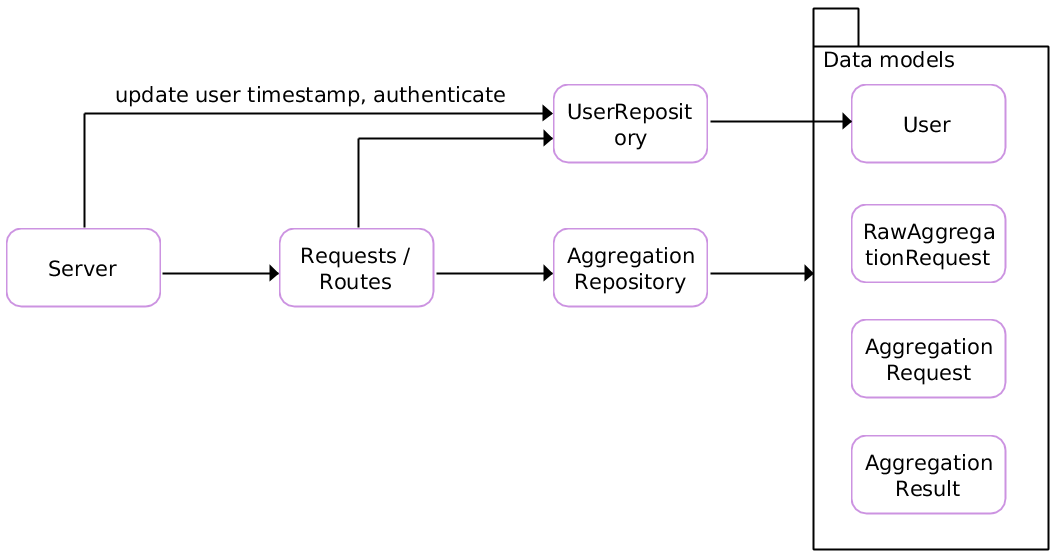
\includegraphics[width=\textwidth]{data/diagrams/server-diagram.png}
\end{figure}

\section{Server Design and Implementation}\label{server}
The server is build using the event-driven node.js verion 10.15.3 leveraging the express\footnote{https://expressjs.com/} web-server framework and using the mocha\footnote{https://mochajs.org/} testing framework in combination with the chai\footnote{https://www.chaijs.com/} assertion library for unit and integration testing. The server is designed using a layered architecture as described in figure \ref{server-architecture}. On the lowest level are the data models which define and verify the data schemes defined in subsection \ref{server-data-model}. The \textit{commonRepository} and the \textit{userRepository} are build on top of those models and persists data in a mongoDB object store. They also handle e.g. transactions where several objects are modified depending on the result of the previous modification (TODO: implement transactions?). The third level provides the logic to be executed for each endpoint defined in \textit{routs.js} while \textit{server.js} on the top level starts the server on the port specified in TODO.environment.json-TODO. It also registers the routes described in section \ref{api}, adds authentication and interacts directly with the \textit{userRepository} in order to update the respective users lastSeen property. Furthermore, it starts a scheduled repeating task to keep the request chain running. This process is described in subsection \ref{request-chain}

\subsection{Data Model}\label{server-data-model}
We organize the data in four collections. The user collection stores the user data which is the public key, the hashed password and "lastSeen" - the timestamp of the last interaction of the user with the server. Aggregation requests are split into two collections. The collection "rawAggregationRequests" stores the initial aggregation request inserted through the admin interface containing the fields start, end, type - the type of the request, the three fields n, value, valueList reused across all aggregations to pass data, the timestamp when the request was filed to the server and a flag indicating whether this request has been started yet\footnote{E.g. when the end data of a newly inserted aggregation request is in the future, the request will be started only when this day has passed}. Upon start of the aggregation request, a list of the 10 most recently active users is retrieved in order to serve this request. The request body is then encrypted with the first users public key and stored in the collection "aggregationRequests". Each time, a user requests an aggregationRequest, proceeds with it and sends the results back to the server, the result is inserted into the database as a new aggregationRequest. The fields of this collection are 
\begin{itemize}
	\item rawRequestId - The id of the related rawRequest. This field is not available through the API.
	\item started\_at - The timestamp, when the request has been started
	\item publicKey - The public key of the user that should proceed this request
	\item nextUser - The public key of the user that will receive the request afterwards. This is necessary so that the user that should proceed this request can encrypt the processed request with the public key of the next user.
	\item previousRequest - The id of the previous request. This is null, if it is the first request in the chain. This is used for the mechanism taking care if a request is not processed by the user it is pending for.
	\item users - the list of public keys of the following users that will proceed with this request. This field is not available through the API.
	\item encryptionKey - A synchronous key, encrypted with the public key of the user the request is aimed at.
	\item iv - the initialization vector used for synchronous encryption and decryption of the actual aggregation request.
	\item encryptedRequest - The actual aggregation request encrypted with the synchronous key.
	\item timestamp - The timestamp when this object has been created.
	\item commpleted - A flag indicating whether this aggregation request has already been proceeded by the respective user and the resulting aggregationRequest has been received by the server.
\end{itemize}
The last collection called "aggregationResults" is used to store the results of an aggregation request. Once there are no more users to serve an aggregationRequest, the last user sends the final data unencrypted to the server where it is stored as an aggregationResult. It contains the same fields as the rawAggregationRequest except the started flag and additionally a field started\_at and timestamp - indicating when the aggregation request referenced through rawRequestId was started and when it was completed.

\subsection(request-chain)\label{request-chain}
//TODO
server.js also invokes a scheduled task which re-routes stale requests where the user has not proceeded with the pending request either due to being offline or due to a problem handling the request. When new aggregation requests are started, the lastSeen timestamp of users is taken into account to exclude users that have not connected for a certain time. Furthermore, the list of users who are selected to serve the new request is ordered by the time the user was last seen.
% !TeX root = ../main.tex
% Add the above to each chapter to make compiling the PDF easier in some editors.
\chapter{Performance and Evaluation}\label{chapter:performance}
\section{Deployment}
The proposed Android application and server have been tested on 16 devices for one week from 30.05.2019 until 06.06.2019. The server was deployed in the IBM Cloud as an 128 MB node.js instance. The database was hosted as a free version at mongodb.com.
We ran each of 8 requests on a daily basis and also for each timespan of several days within this period. The raw results can be found at XXX\footnote{Only 7 of the 8 aggregations are available as it is. The results of aggregation 8 where modified in order to protect user priacy}. We used this testing period also to improve the performance of the server as well as the Android application and to find and remove bugs.

\section{Results}
The results support our hypothesis that data can be analyzed decentrally and that aggregated data can be published without any privacy concerns. The aggregations of mean values clearly leave no doubt about full privacy protection as there even is no personal data involved anymore. The listing of mean values of average number of steps per participant allows for more advanced statistical analysis while at the same time the values cannot be mapped to persons. Even when conducting the same request twice, due to users being chosen dynamically, one could most probably see if the same user participated in the second request but nothing else. When aggregating over another time period (that might have an intersection with the other one), there is not even the chance to identify whether the same user participated in both aggregations. As requests are started not at the same time (TODO!!!), and users are in a future setting allocated dynamically to the request, there is also no chance to link the data from different aggregations. From the number of steps one could infer the time somebody spent walking, but as it is not given whether the steps where conducting walking, running or both, this linking would result in a very poor performance and also only reveal that to a very low probability, the user with X steps in one aggregatioin is the same user spending X minutes walking the same day. 
The listing of trajectories created a dataset that clearly shows the vulnerability highlighted in XX and XX. Nevertheless, this is no aggregation but just a collection of raw data with stripped of identifiers and timestamps anonymized to a daily basis. The results show clearly that our setup is sufficiently accurate to field test the other aggregations proposed in XX and further prove our thesis. The data shows, that e.g. A change of transportation system can clearly be identified. 
% !TeX root = ../main.tex
% Add the above to each chapter to make compiling the PDF easier in some editors.
\chapter{Conclusion and Discussion}\label{chapter:conclusion}
\section{Conclusion}

\subsection*{RQ1: How is aggregation of location data possible without raw data being accessible to anybody but the owner?}
We developed and field tested an approach that allows for decentral aggregation of data that preserves the privacy of users. Due to fast-changing IP-addresses, stable P2P on mobile devices is currently either limited to WIFI and Bluetooth connections or limited by the Bandwidth and cost of SMS. Hence, we proposed a solution based on the assumption of a trusted server that forwards messages between the different Android mobile phones. Nevertheless, the messages are encrypted and only the target device can encrypt the message, as long as the server is not compromised. On the mobile devices, raw data i.e. GPS data, steps and detected activities is collected and locally aggregated through an Android application. This locally aggregated data is then used to serve aggregation requests initiated and forwarded by a central server but the raw data and the locally aggregated data itself is never send away from the device. Thus, considering the assumption of a trusted server and trusted devices, we propose a solution that indeed manages to aggregate locational data without the raw data being exposed from the collecting devices.
%This highlights that we had to base our solution on the assumption of a trusted server and trusted devices.

\subsection*{RQ2: What types of aggregations can be published?}
We used the proposed setup to compute mean values for the number of steps and the time spent in the activities walking, in a vehicle, biking and running across all aggregation participants in our field testing. In Chapter \ref{chapter:performance} we presented and discussed the results. We found that we had no chance to infer any information about the participating users from the mean values. During field testing we also collected lists of individual mean values for the average number of steps per day. These lists enable the computation of e.g. median value or distribution function. We have not found any trivial possibility to infer any information about the identity of the user. Furthermore, it does not seem feasible to link values from two subsequent aggregations to the same user. We further showed in Section \ref{inference} that it seems unlikely to infer that the same user participated in two different types of aggregations e.g. the computation of the average number of steps and the computation of the average time spent walking.

\subsection*{RQ3: Are inference attacks similar to inference attacks on anomyized data sets possible?}
We found in Chapter \ref{chapter:performance} that it is possible to infer that the same user participated in different aggregations that overlap regarding the covered timespan. Nevertheless, this is on the one hand based on the fact that the user did not provide data for the days that were only covered by one of both aggregations. On the other hand, we do not see a possibility to infer further information e.g. the identity of the user from this inference.

\section{Limitations}
As stated in Chapter \ref{chapter:method}, our approach is based on trust among the clients and the server. Nevertheless, while e.g. Kajino et al. \parencite{crowdsourcing} face the same problems in case of a compromised server - namely that the server can create artificial participants and thus obtain the raw values from each user, our setup is more general, allows for more complex aggregations and can be adapted to work via P2P if devices are locally close to each other or P2P generally becomes possible on mobile devices. Also, trust can be established through various means. Pouryazdan et al. \parencite{pouryazdan2017quantifying} propose a reputation score and Weng et al. \parencite{li2018crowdbc} propose a solution through blockchain technology.

In addition, the field testing should be repeated with more users and more aggregations in order to obtain a larger data set. We do not expect the findings to be any different though, because the key to publication without privacy concern seems to be that never a GPS location is included in the publication. Only in the question of the aggregation itself a GPS location might be referenced e.g. by limiting the area of the aggregation as proposed in Chapter \ref{chapter:method}.

\section{Future Work}
In order to continue this research, the provided setup was carefully designed to allow for very flexible adaptability and extensibility. Some parts proposed in Chapter \ref{chapter:method} were not implemented in this research due to scope limitations. The implementation of these features e.g. the proposed but not yet implemented aggregations, limiting the area of an aggregation and the incorporation of the findings of our field test are a good starting point for future work. In addition, the following Subsections show options of improvement and further research in the respective areas of the Android application and the server itself as well as more conceptual advancements.

\subsection{Android Application}\label{future-android}
There is a list of promising rather technical improvements to the Android application. They are listed as open issues at the public GitHub repository and should be resolved or implemented but were out of the scope of our research. Furthermore, our experience showed that some essentials as e.g. providing a nice information screen to the user when opening the application or showing the own locally aggregated data would boost participation. The aggregations publicly available on the server could also be used to show a comparison of e.g. the personal number of steps to the average or the median. Also making the application available through the play store would be a great relief for the user and simplify the installation process a lot and in addition enable the roll-out of updates and client-side fixes during field testing. Also the option to delete local data after some time or export it might increase user adoption. Furthermore, the user could be asked to specify home and work location which are then stored locally. This spares having to locally infer these locations while enabling better aggregations and also even more guaranteed privacy protection.

\subsection{Server}
The main possibilities for improvement concerning the server center around dealing with the problem of not available users blocking the aggregation chain. Dynamically selecting the subsequent user at every step and not selecting the whole list of users upfront would allow for benefits from taking the probability of the user being active into account. Nevertheless, no matter when the users are determined, it has to be investigated that the selection of users for an aggregation is does not lead to a bias in the aggregation result. Furthermore, encrypting an aggregation not only for one but for several subsequent users\footnote{Once one of these users processes the aggregation, the aggregation requests to the other users become disabled} would generate some redundancy overhead but yield fewer problems due to not responding users.
Some other rather technical improvements like e.g. pre-populating aggregation requests in order to hinder the first users in the chain from inferring the data of the previous user with a high probability and cleaning the aggregation result from this pre-filling upon completion of the aggregation can be found in a list of issues at the respective GitHub repository as described in Section \ref{future-android}.

\subsection{Related Research Areas}
Our research is very close to some related research areas e.g. decentral computation. Our setup can be used as well as a base for research in this area where problems might be solved locally and collected by the server afterwards and the pieces put together still with anonymity provided for the users. Similarly, our setup would also allow for pre-populating device databases with artificially generated or elsewhere obtained data e.g. in order to verify whether aggregated results provide the same insights as one could obtain by analyzing a raw data set.
The application can also be modified to be a framework that can easily be incorporated into other apps especially in order to allow for a broader user base in research projects.
Trust is a basic assumption of our framework. A whole area of research e.g. blockchain technology or credit systems or use of third parties deal with the question of how to establish or verify trust.

\section{Reproducability Considerations}
The ReadMe file of the server \parencite{readme-server} provides detailed instructions of how to install and run the server proposed in our work and where in the code the url of the database has to be provided. Section \ref{deployment} gives an example of a deployment option but the software can be installed on any server. The Android application can be installed on any compatible device\footnote{As stated in Section \ref{android-app}, the minimum required API level is 19 and Google Play Services has to be installed on the device.} using the \textit{.apk} file included in the realease \parencite{final-version-app}. Once the server is running, the application automatically registers with the server upon successful installation and granting of location access. Aggregations can be initiated using the API endpoint detailed in Section \ref{api} and Fig. \ref{insert-sample}.
The results obtained should resemble the results obtained in our work. Nevertheless, the actual data will vary accordingly to the activity of the participants.

\begin{appendices}
	% !TeX root = ../main.tex
% Add the above to each chapter to make compiling the PDF easier in some editors.
\chapter{Data Usage Screenshots}
\begin{center}
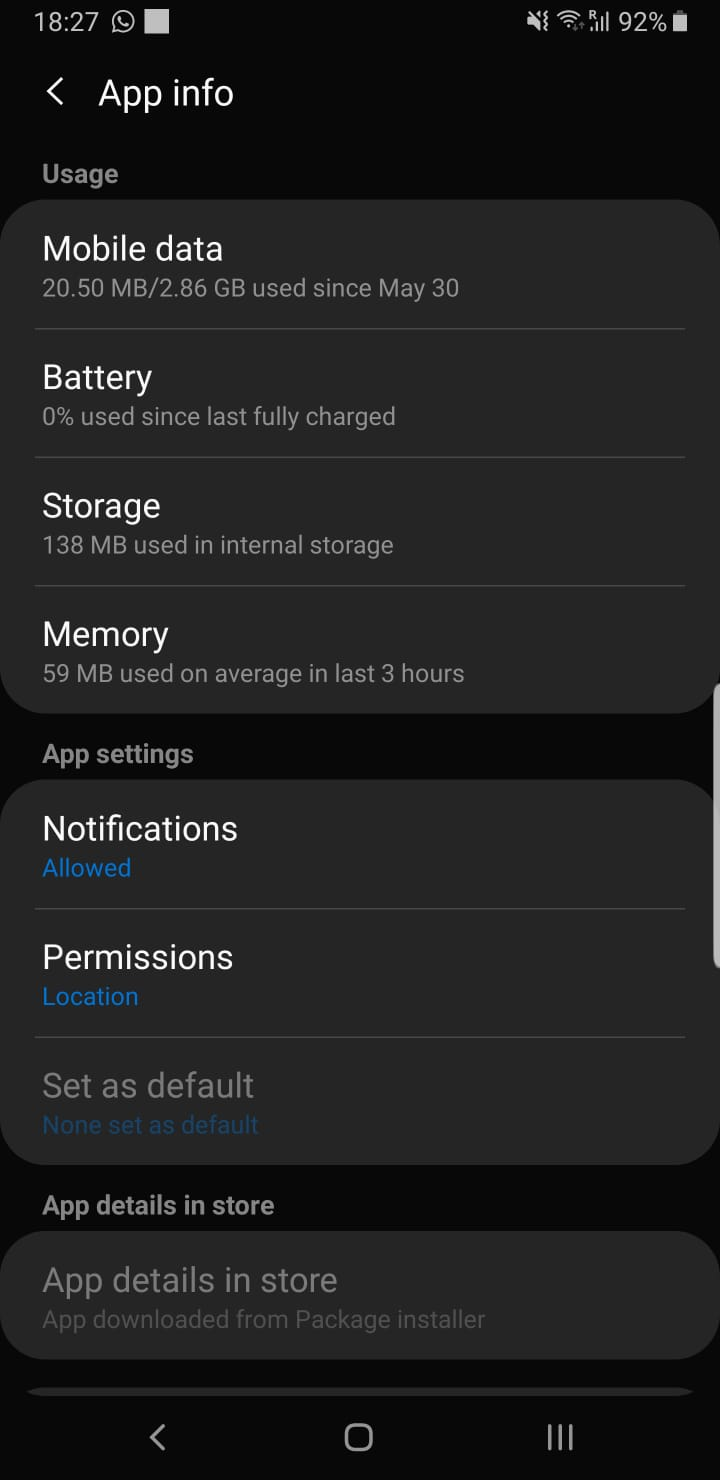
\includegraphics[width=0.5\textwidth]{data/data-usage/data-usage1.jpeg}
\end{center}
\begin{center}
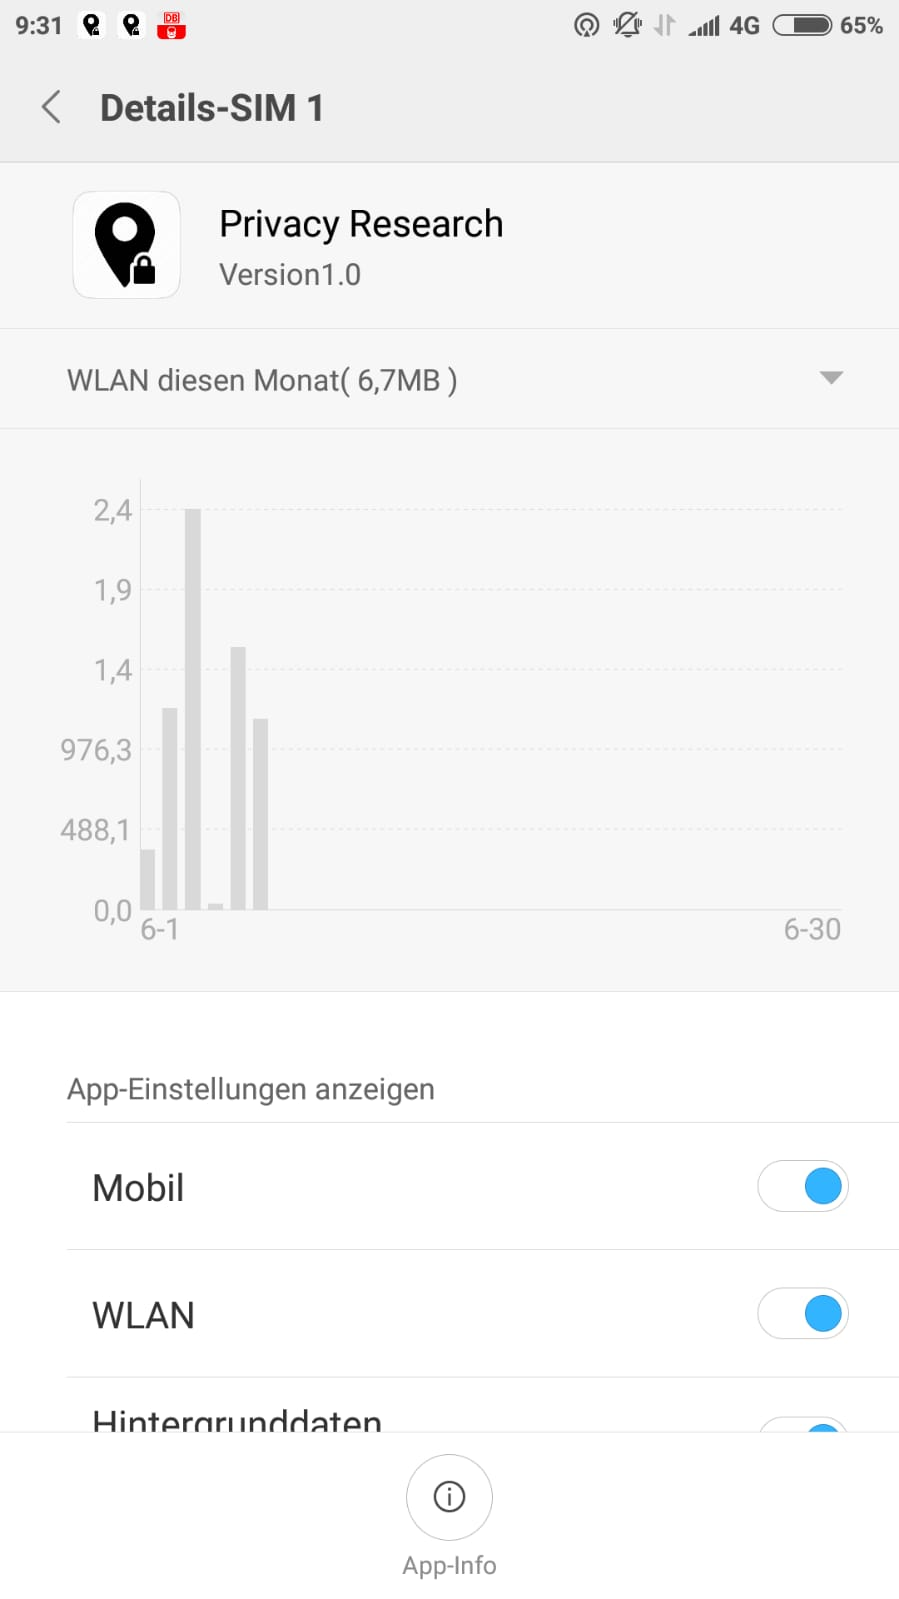
\includegraphics[width=200pt]{data/data-usage/data-usage2-1.jpeg}
\end{center}
\begin{center}
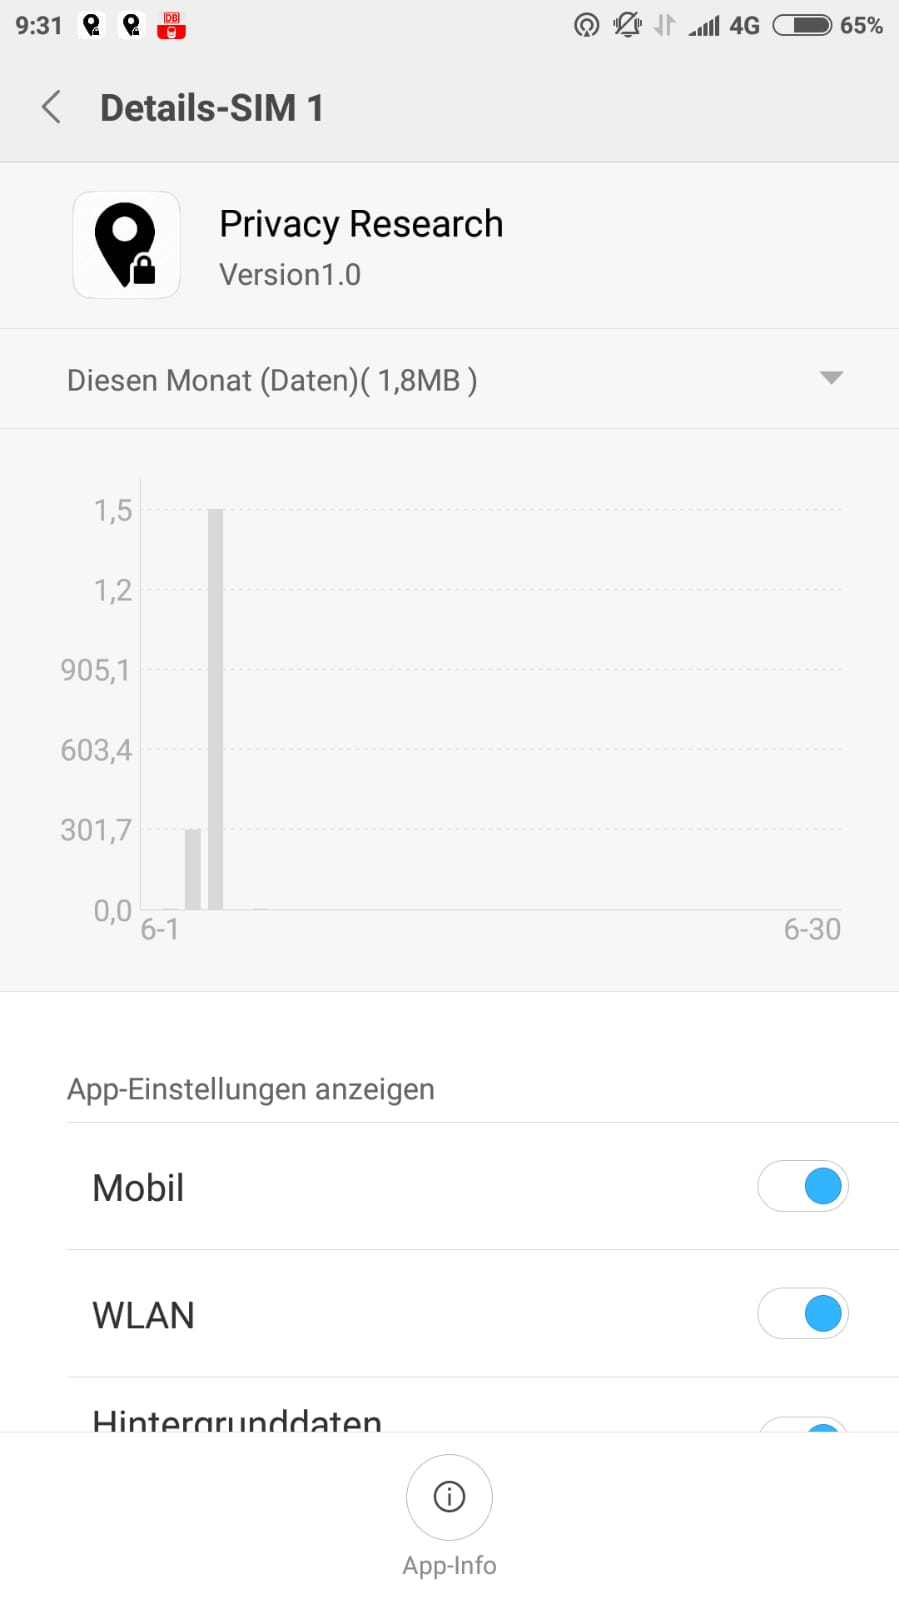
\includegraphics[width=200pt]{data/data-usage/data-usage2-2.jpeg}
\end{center}
\begin{center}
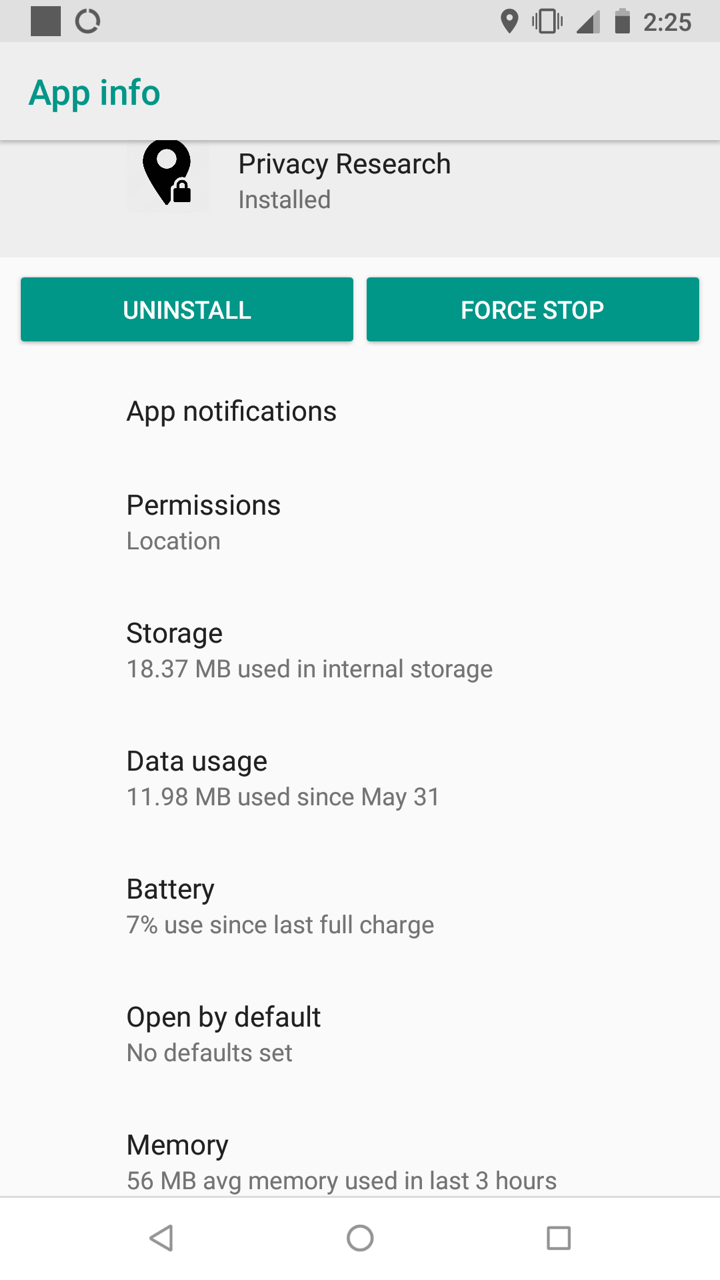
\includegraphics[width=200pt]{data/data-usage/data-usage3.png}
\end{center}
\begin{center}

\includegraphics[width=200pt]{data/data-usage/data-usage4.jpeg}
\end{center}
\begin{center}
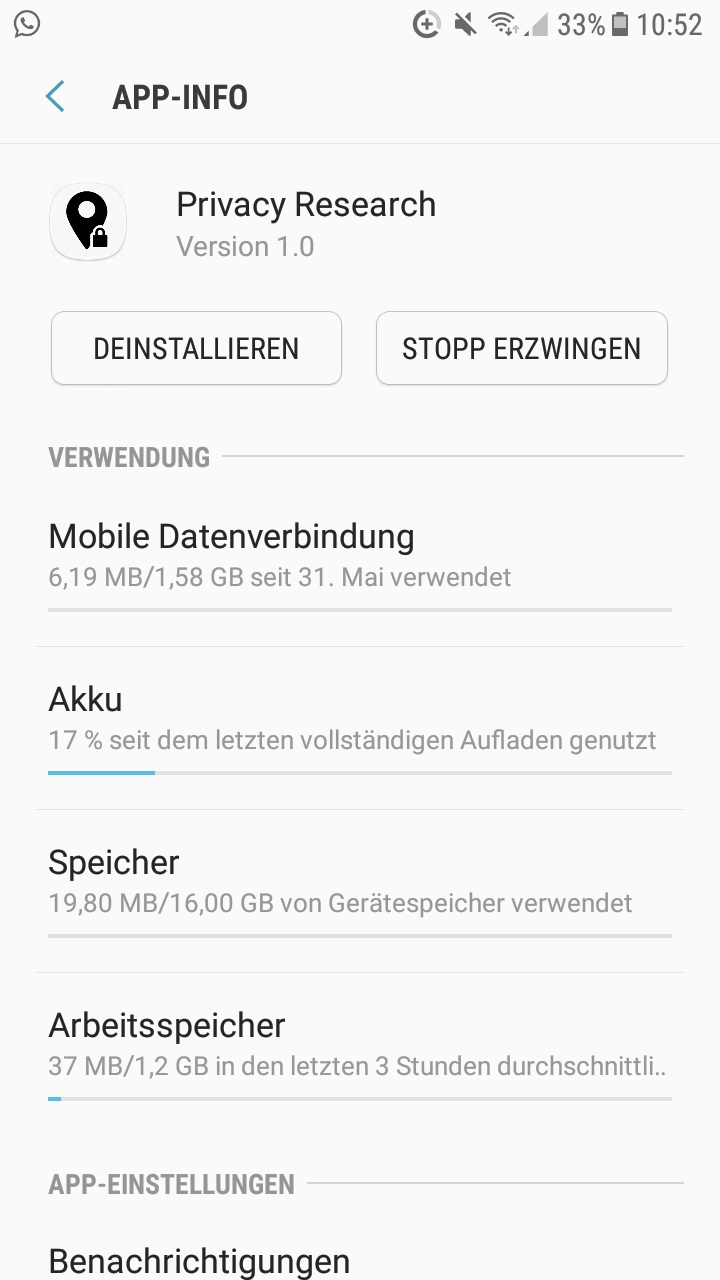
\includegraphics[width=200pt]{data/data-usage/data-usage5.jpeg}
\end{center}
\begin{center}
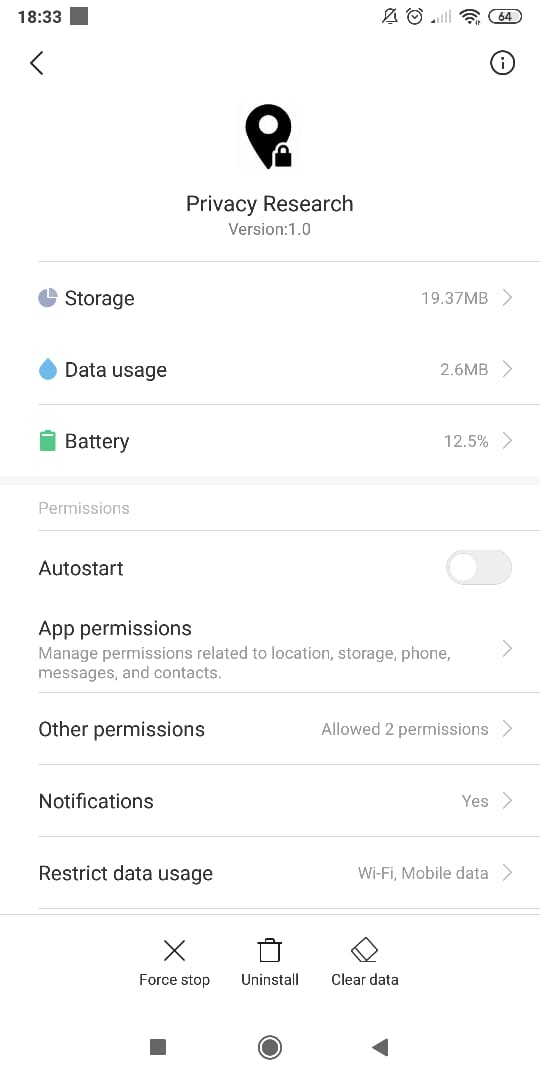
\includegraphics[width=200pt]{data/data-usage/data-usage6.jpeg}
\end{center}
\begin{center}
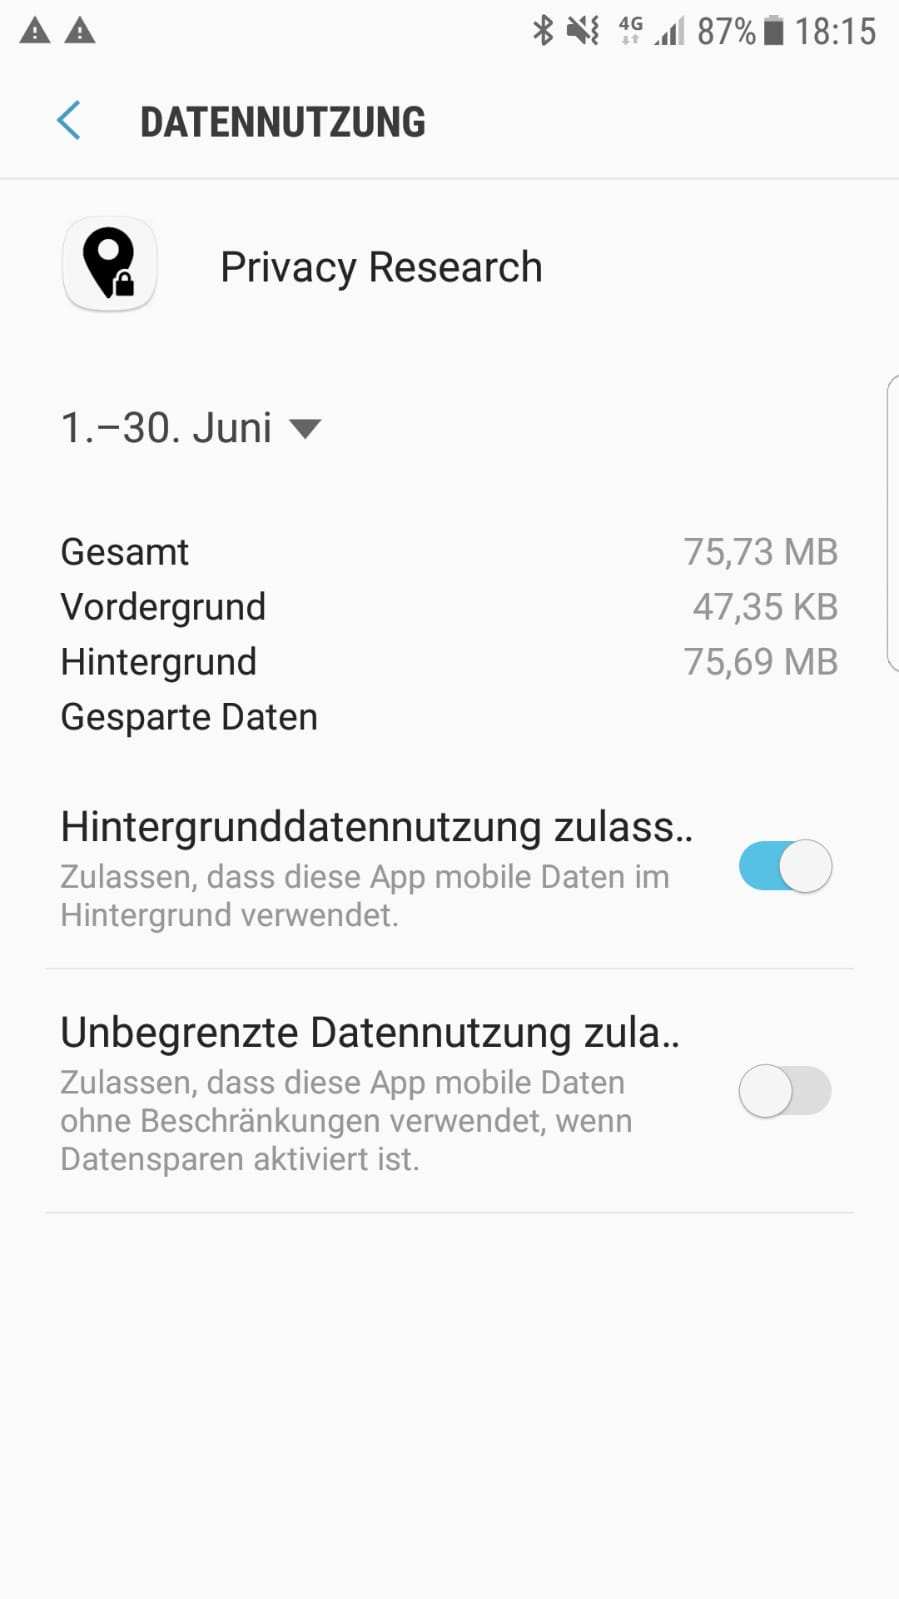
\includegraphics[width=200pt]{data/data-usage/data-usage7.jpeg}
\end{center}
\begin{center}
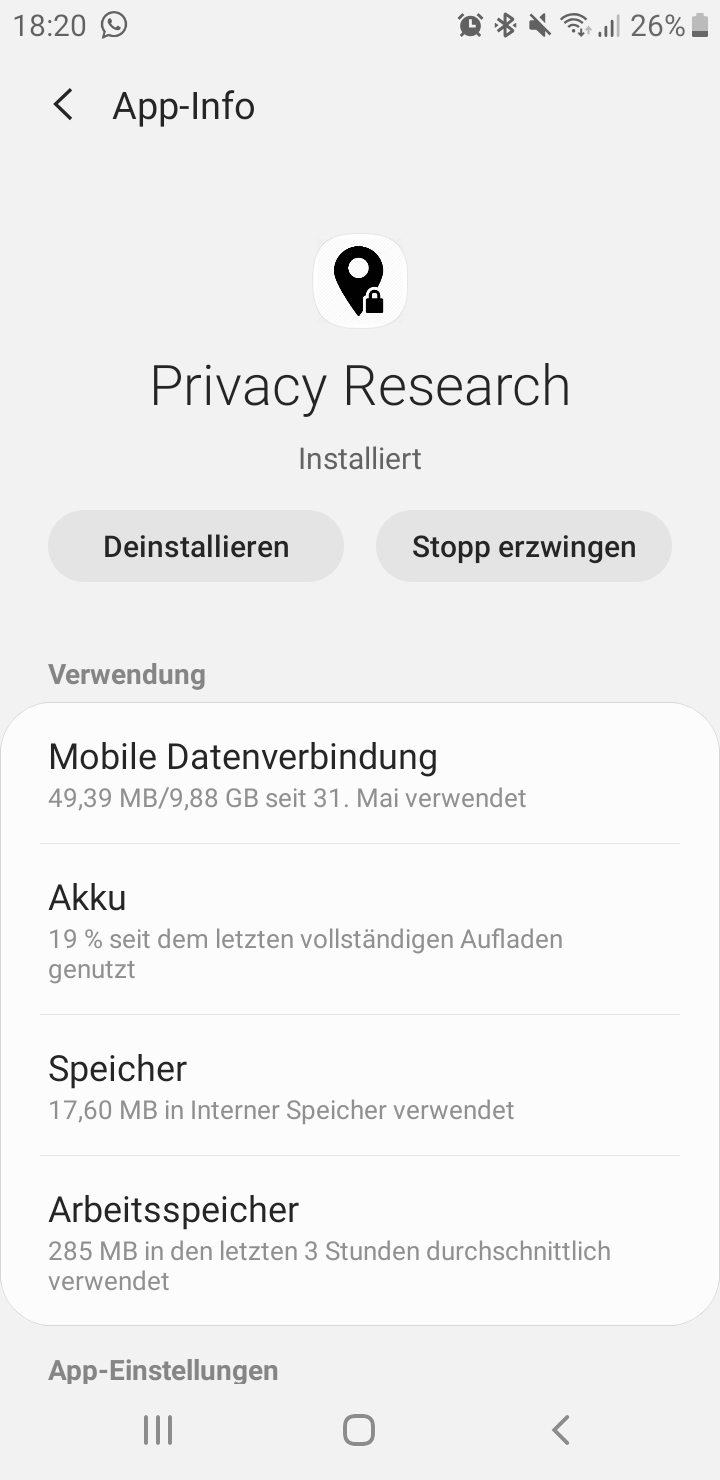
\includegraphics[width=200pt]{data/data-usage/data-usage8.jpeg}
\end{center}
\begin{center}
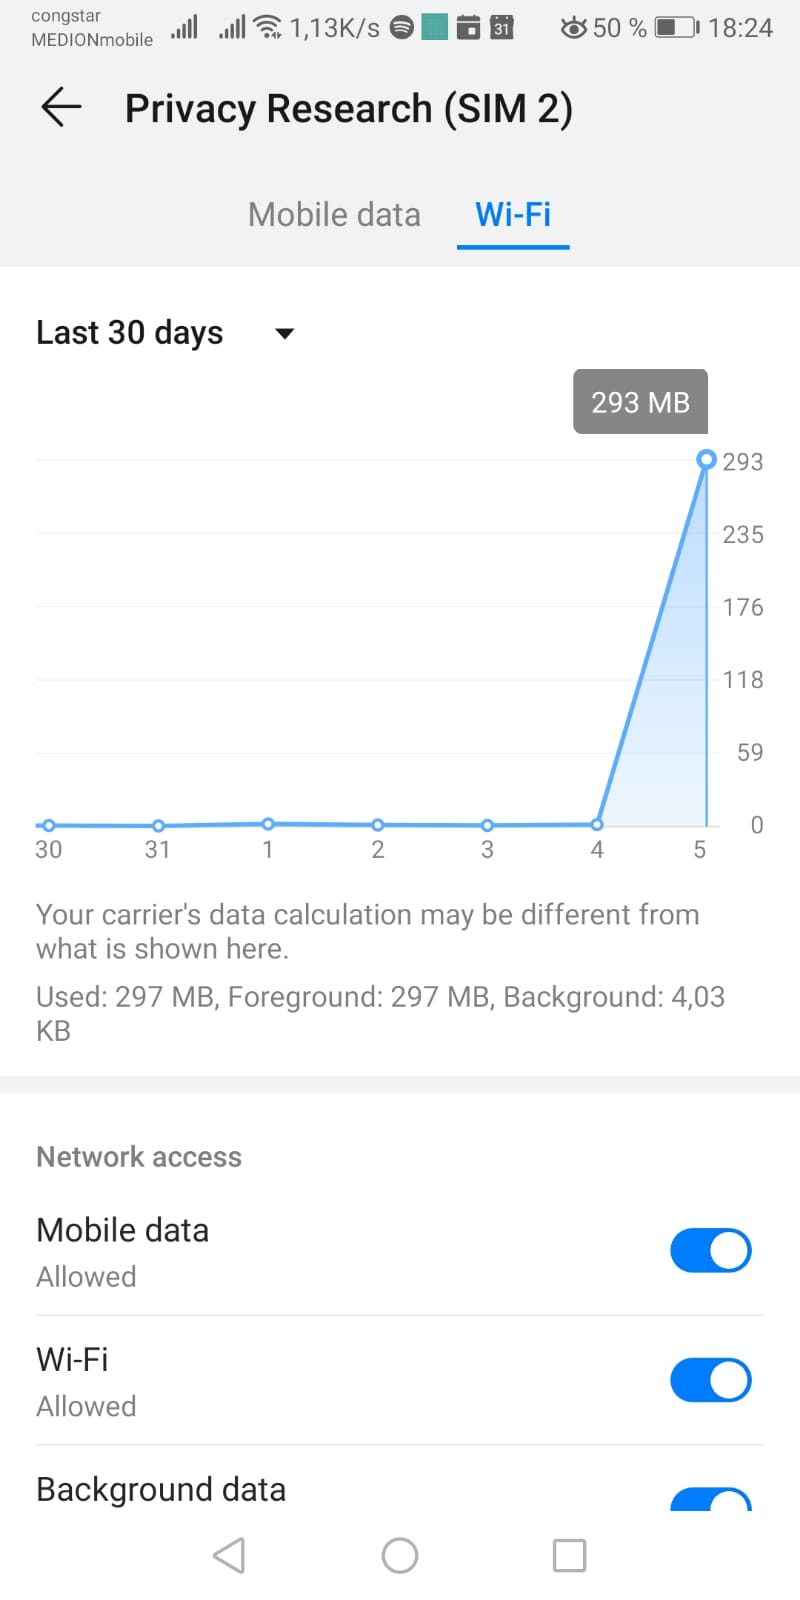
\includegraphics[width=200pt]{data/data-usage/data-usage9-1.jpeg}
\end{center}
\begin{center}
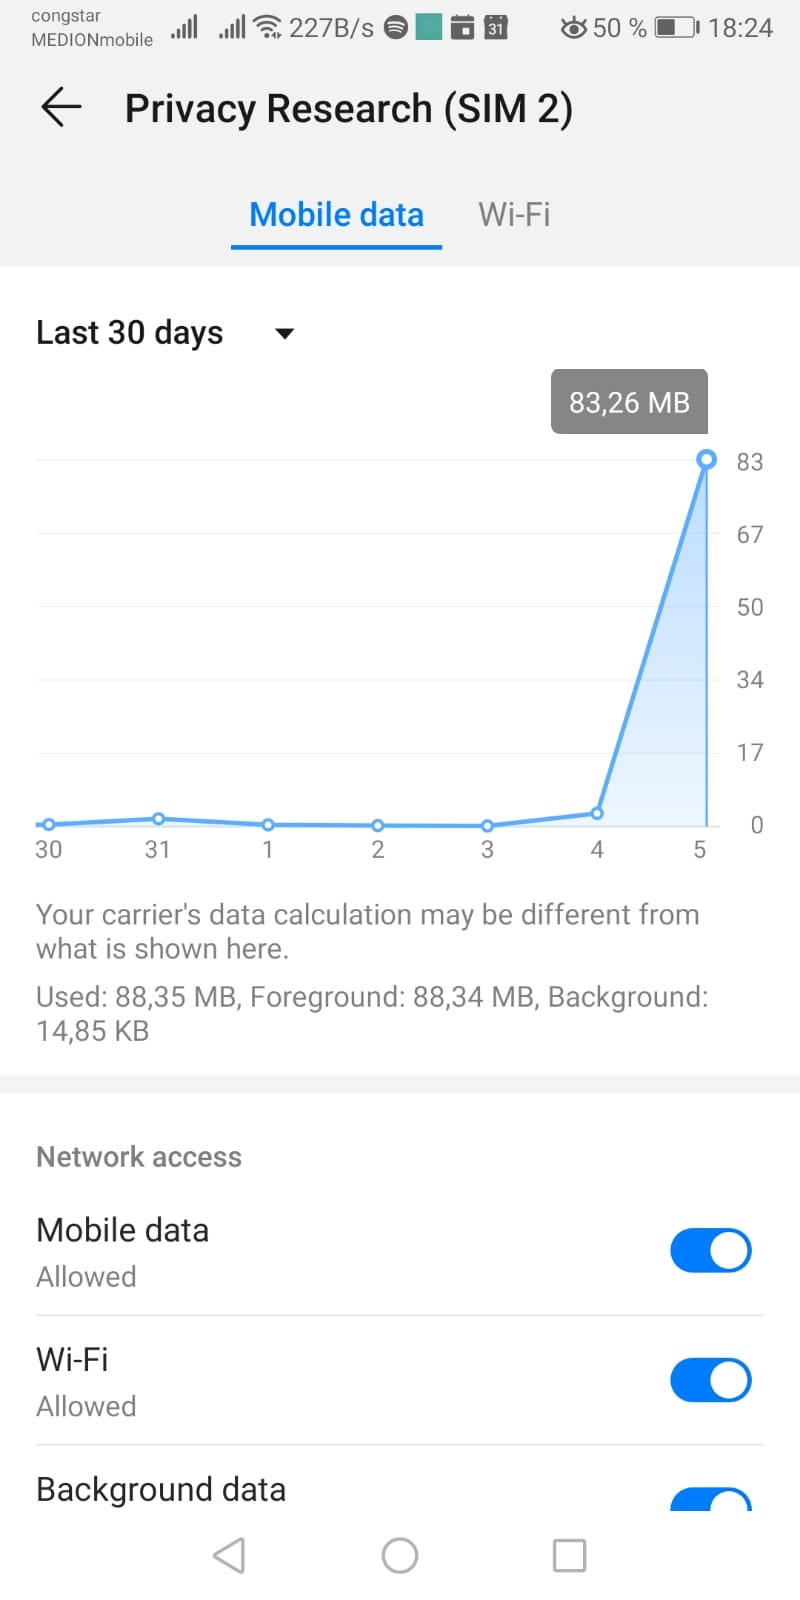
\includegraphics[width=200pt]{data/data-usage/data-usage9-2.jpeg}
\end{center}
\end{appendices}

\microtypesetup{protrusion=false}
\listoffigures{}
\listoftables{}
\microtypesetup{protrusion=true}
\printbibliography{}

\end{document}